\section*{frac\_shared is not the informative statistic}

A second result fell out of the pairs included only to fix the null: sharing
causal \emph{variants} is nearly free, and carries little information on its
own.

GGT $\times$ bilirubin and SHBG $\times$ ALP were chosen as unrelated pairs of
polygenic traits. They share 63\% and 71\% of the smaller causal set --- and
their shared effects correlate at $-0.05$ and $-0.06$. Sitting at nearly the
same \texttt{frac\_shared}, gout $\times$ CRP and cystatinC $\times$ CRP
correlate at $+0.37$ and $+0.34$. For traits that are each causal at tens of
thousands of variants, substantial overlap of the causal \emph{sets} is close to
the default, and it is the \emph{direction} of the shared effects that
discriminates.

The qualification matters: over the whole range \texttt{frac\_shared} is not
uninformative --- it runs from $0.39$ at the bottom of the scale to $1.00$ at
the top. What it cannot do is separate pairs in the middle, which is where most
real pairs fall.

\begin{figure}[H]
\centering
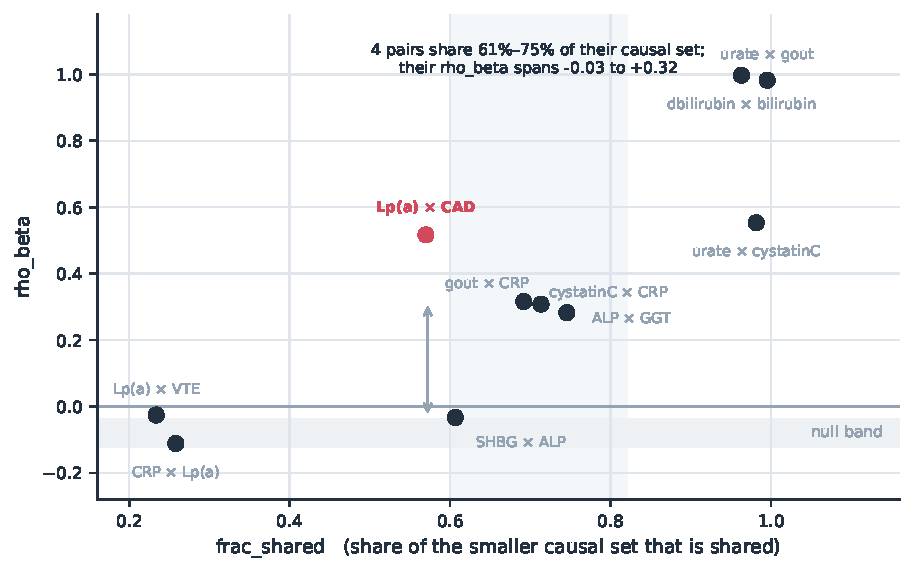
\includegraphics[width=\linewidth]{figures/frac-shared.pdf}
\caption{\texttt{frac\_shared} against \texttt{rho\_beta}. Across the full
range the two are plainly associated --- it is the middle that cannot be
resolved. Inside the shaded column, five pairs share 63--80\% of their causal
set while their \texttt{rho\_beta} spans $-0.06$ to $+0.37$. Lp(a) $\times$ CAD
sits low on the horizontal axis because Lp(a) has few causal variants at all,
which is the point: a small shared set with a consistent direction. The
horizontal band marks where the four below-zero pairs fall; it is descriptive,
not a test.}
\end{figure}

This matters for how the overlap summary should be read. \texttt{n\_shared} and
\texttt{frac\_shared} describe how much of the architecture is common;
\texttt{rho\_beta} describes whether the common part agrees. Only the second
distinguishes the pairs here.
